\section{Basic Hardware Construction in Chisel}
The Chisel constructs presented in the previous section are adequate
for most hardware circuits. We have in fact built an entire floating
point library using only those constructs. Occasionally, users might
want to leverage syntax available in a target backend from within
Chisel. Suppose for example that a user is having Chisel target a
backend that has support for highly optimized FFT circuits. One way to
leverage this feature is to introduce a new type of {\tt Node} into
Chisel that maps directly to that syntax in the backend. This section
will show how ListLookup, Vec, and When Nodes are implemented to
target Verilog's case statements, arrays, and if statements
respectively.

\subsection{ListLookup}
\begin{figure}[hb]
\centering
  \begin{subfigure}[t]{0.48\textwidth}
  \centering
  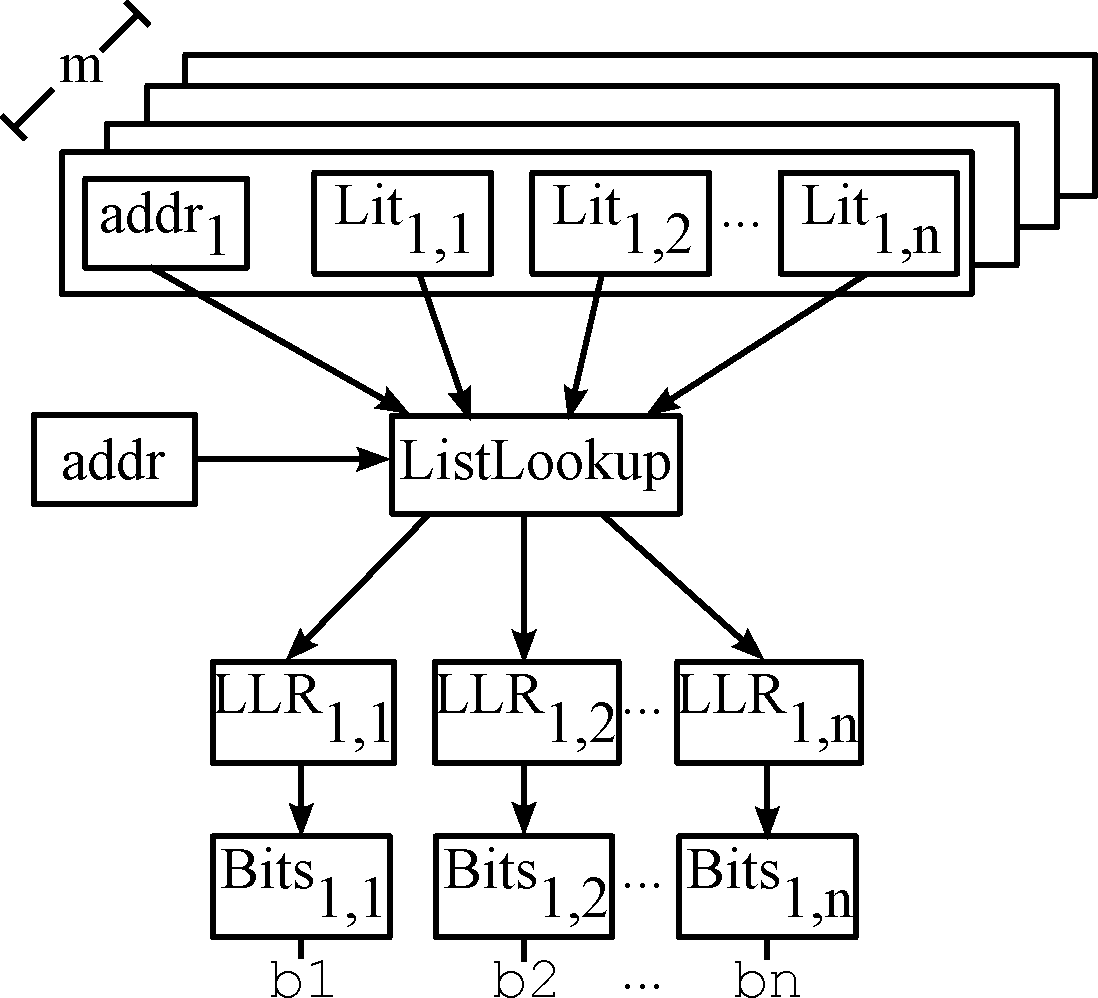
\includegraphics[width=\textwidth]{figures/listlookupnode.pdf}
  \caption{ListLookup Node}
  \label{fig:llnode}
  \end{subfigure}
  \hfill
  \begin{subfigure}[t]{0.48\textwidth}
  \centering
  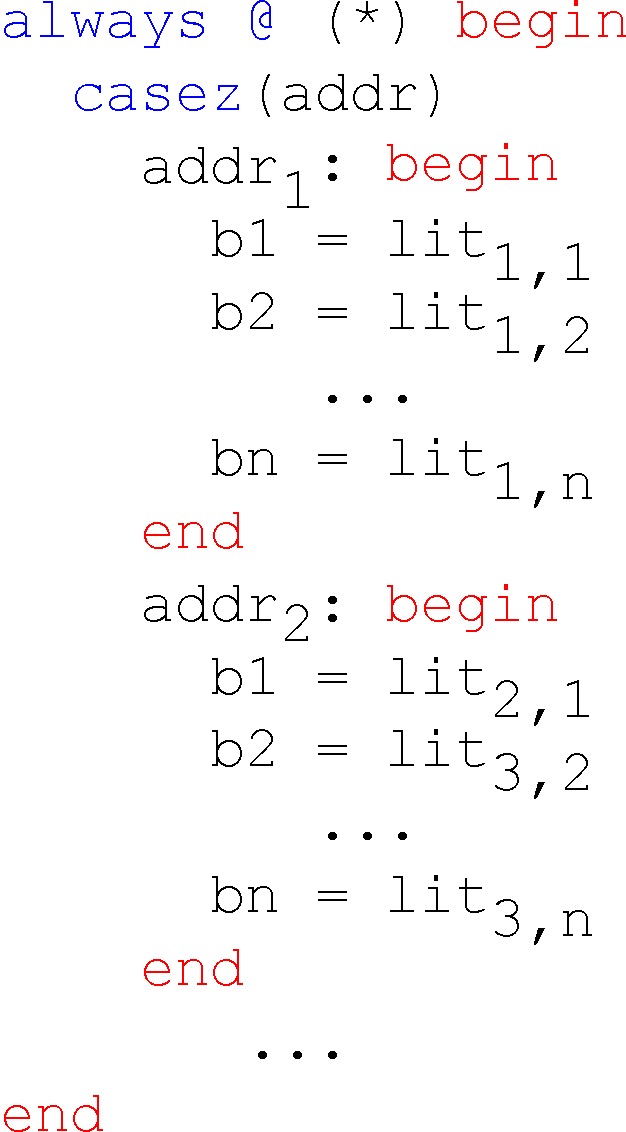
\includegraphics[width=0.5\textwidth]{figures/listlookupv.pdf}
  \caption{Generated ListLookup Code}
  \label{fig:llv}
  \end{subfigure}
\caption{ListLookup}
\label{fig:ll}
\end{figure}

Figure~\ref{fig:llnode} shows the new nodes that are required to
support Verilog's case statement in Chisel and Figure~\ref{fig:llv}
shows the corresponding Verilog code generated from the graph. 

\textbf{ListLookup Node}. The inputs to this node is an address and a
list of tuples {\tt ($a_i$, $lits_i$)} where {\tt $lits_i$} is a list
of a literals. This node is different from other nodes in that it does
not have an entry for {\tt emitDec} and {\tt emitRef}. The only code
generation function it fills out is the {\tt emitDef} function which
generates the case statemetns in Figure~\ref{fig:llv}. The ListLookup
generates a case statement for every {\tt ($a_i$, $lits_i$)} tuple
where each case statements will have an assignment for each literal in
{\tt $lits_i$}. The address input to the ListLookup is used as the
lookup address into the case statement and the {\tt $a_i$}'s are used
to match against the address.

\textbf{ListLookupRef Node}. Creating a new {\tt ListLookup} will not return
the {\tt ListLookup} to the user, rather, a list of 
{\tt ListLookupRef} nodes are returned instead. The length of the 
{\tt ListLookupRef} list matches the length of {\tt $lits_i$}. 
{\tt ListLookupRef} nodes do not have an entry for {\tt emitDef} since
the assignments to these nodes are actually done in the {\tt emitDef}
of a {\tt ListLookup} node.


\subsection{Vec}
\begin{figure}[hb]
\centering
  \begin{subfigure}[t]{0.48\textwidth}
  \centering
  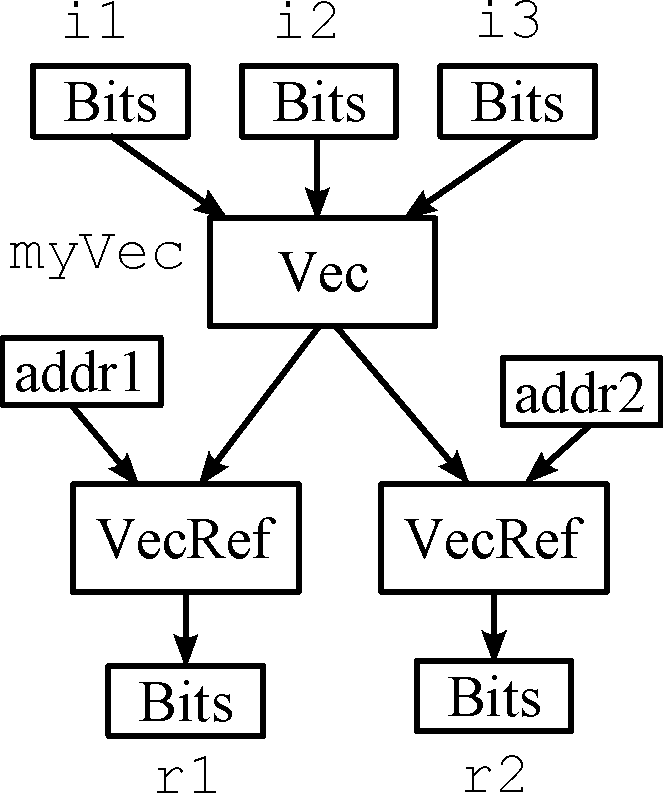
\includegraphics[width=0.5\textwidth]{figures/vecnode.pdf}
  \caption{Vec Node}
  \label{fig:vecnode}
  \end{subfigure}
  \hfill
  \begin{subfigure}[t]{0.48\textwidth}
  \centering
  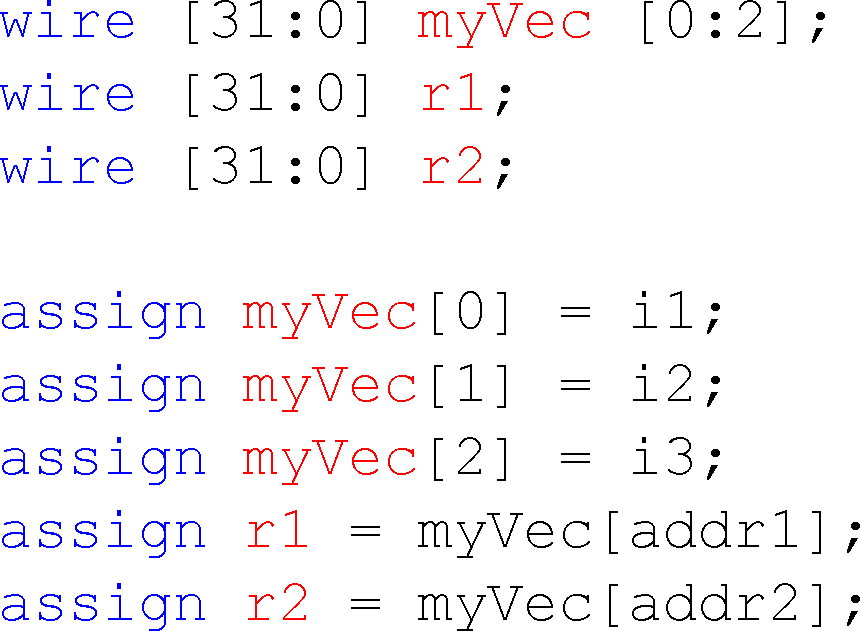
\includegraphics[width=0.7\textwidth]{figures/vecv.pdf}
  \caption{Generated Vec Code}
  \label{fig:vecv}
  \end{subfigure}
\caption{vec}
\label{fig:vec}
\end{figure}

Figure~\ref{fig:vecnode} shows the nodes that implement a
2-dimensional Verilog array in Chisel and Figure~\ref{fig:vecv} shows
the generated Verilog code.

\textbf{Vec Node}. The {\tt Vec} node maps directly to the 2-D Verilog
array. Users instantiate this node with the desired number of entries
and then populate the node using {\tt :=}
assignments. Figure~\ref{fig:vecnode} shows a 3-entry {\tt Vec} where
the user has connected {\tt i1-3} to the {\tt Vec}. The width of a
{\tt Vec} node is inferred to be the maximum width of its inputs (in
this example, 32-bits wide). {\tt Vec}'s {\tt emitDec} function will
return the string
\begin{align*}
\centering
\text{\tt{wire [width-1:0] vec\_name [0:entries-1];}}
\end{align*}
where {\tt vec\_name} is the name of the node, {\tt width} is the
inferred width, and {\tt entries} is the number of entries in the
{\tt Vec}. The {\tt emitDef} function emits an assign statement for
each entry in the Vec.

\textbf{VecRef Node}. After instantiating and populating the Vec,
users will want to access the {\tt Vec} with dynamic addresses. Each
access with a new address will make a new {\tt VecRef} node. The
inputs to a {\tt VecRef} node are an address and a 
{\tt Vec} and its inferred with is the width of its input
{\tt Vec}. Figure~\ref{fig:vecnode} two {\tt VecNode} made from
accessing the same {\tt Vec} with two different addresses. 
{\tt VecRef}'s {\tt emitDec} simply declares the name and width of the
node. Its {\tt emitDef} entry will return the string
\begin{align*}
\centering
\text{\tt{assign ref\_name = vec\_name[addr];}}
\end{align*}
where {\tt ref\_name} is the name of the {\tt VecRef} node, 
{\tt vec\_name} is the name of the {\tt Vec} and {\tt addr} is the
address.
\subsection{When}
